\documentclass[12pt]{beamer}
\usepackage[spanish]{babel}
\usepackage{graphicx}
\usepackage{amsmath}
\usepackage{booktabs}
\usepackage{caption}

\usetheme{Madrid}
\title[Métodos de Optimización]{Análisis del Producto Bruto Interno (PBI) mediante Regresión Lineal y Optimización con Optuna}
\subtitle{Curso: Métodos de Optimización - Universidad Nacional del Altiplano}
\author[Jefry Erick Quispe Ramos]{Jefry Erick Quispe Ramos}
\date{\today}

\begin{document}

\begin{frame}
    \titlepage
\end{frame}

% --- Introducción ---
\section{Introducción}
\begin{frame}{Introducción}
    \textbf{Tema:} Producto bruto interno y demanda interna (variaciones porcentuales anualizadas) - PBI.\\
    \textbf{Objetivo:} Modelar la tendencia del PBI minero (2000-2025) usando:
    \begin{itemize}
        \item Regresión lineal simple.
        \item Optimización de hiperparámetros con Optuna.
    \end{itemize}
    \textbf{Datos:}
    \begin{itemize}
        \item 303 observaciones mensuales.
        \item Variables: Fecha (Ene00-Dic25) y Variación \% anualizada.
    \end{itemize}
\end{frame}

% --- Metodología ---
\section{Metodología}
\begin{frame}{Metodología}
    \textbf{1. Limpieza y Exploración:}
    \begin{itemize}
        \item Conversión de fechas (ej: \texttt{Ene00} $\rightarrow$ \texttt{2000-01-01}).
        \item Creación de variable numérica para tiempo (\texttt{Año\_num}).
    \end{itemize}
    
    \textbf{2. Regresión Lineal:}
    \begin{equation*}
        y = \beta_0 + \beta_1 X \quad \text{(PBI vs. Tiempo)}
    \end{equation*}
    
    \textbf{3. Optuna:}
    \begin{itemize}
        \item Optimización del grado de polinomio (1 a 5) para minimizar el MSE.
    \end{itemize}
\end{frame}

% --- Resultados: Exploración ---
\section{Resultados}
\begin{frame}{Exploración de Datos}
    \begin{exampleblock}{Estadísticas Descriptivas}
        \begin{tabular}{lrr}
            \toprule
            \textbf{Métrica} & \textbf{Valor} \\
            \midrule
            Media & 4.27 \\
            Desviación estándar & 6.80 \\
            Mínimo & -39.27 \\
            Máximo & 59.84 \\
            \bottomrule
        \end{tabular}
    \end{exampleblock}
    
    \begin{figure}[ht]
        \centering
        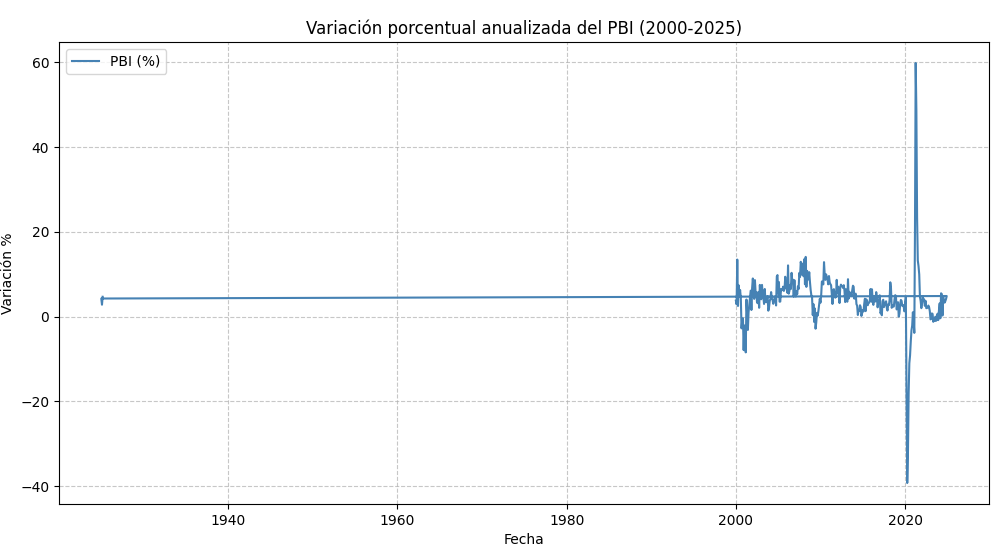
\includegraphics[width=0.6\textwidth]{1grafico.png} % Reemplaza con tu gráfico
        \caption{Serie temporal del PBI minero (2000-2025).}
    \end{figure}
\end{frame}

% --- Resultados: Regresión Lineal ---
\begin{frame}{Regresión Lineal Simple}
    \textbf{Resultados:}
    \begin{itemize}
        \item Pendiente: $-0.0474$ (tendencia leve decreciente).
        \item Intercepto: $99.6863$.
        \item MSE: $45.7508$.
        \item $R^2$: $0.0062$ (baja explicación lineal).
    \end{itemize}
    
    \begin{figure}[ht]
        \centering
        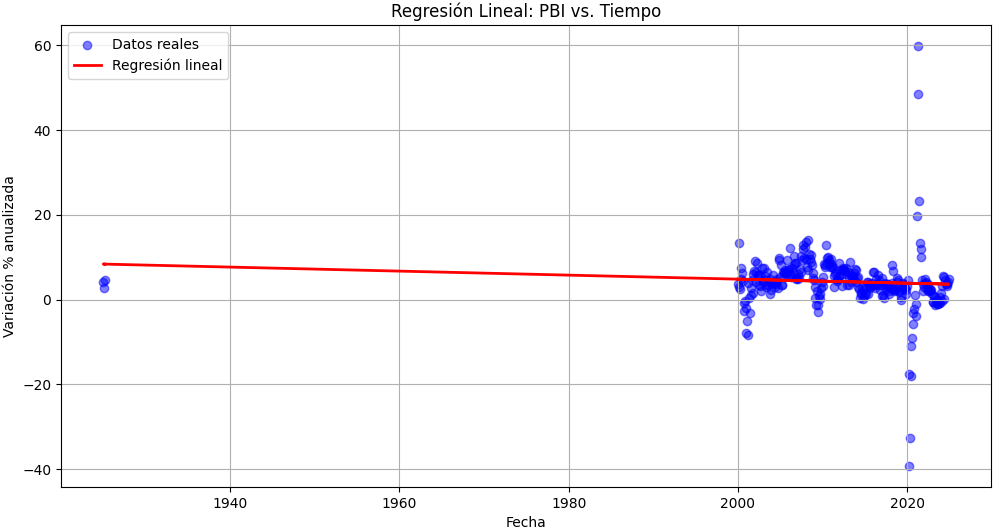
\includegraphics[width=0.6\textwidth]{2grafico.png} % Reemplaza con tu gráfico
        \caption{Ajuste de la regresión lineal.}
    \end{figure}
\end{frame}

% --- Resultados: Optuna ---
\begin{frame}{Optimización con Optuna}
    \textbf{Mejor modelo encontrado:}
    \begin{itemize}
        \item Grado polinomial óptimo: \textbf{5}.
        \item MSE mínimo: \textbf{42.9518} (mejor que el lineal).
    \end{itemize}
    
    \begin{block}{Interpretación}
        Un polinomio de grado 5 captura mejor la variabilidad no lineal del PBI que el modelo lineal ($\text{MSE}_{\text{lineal}} = 45.7508$).
    \end{block}
    
    \begin{figure}[ht]
        \centering
        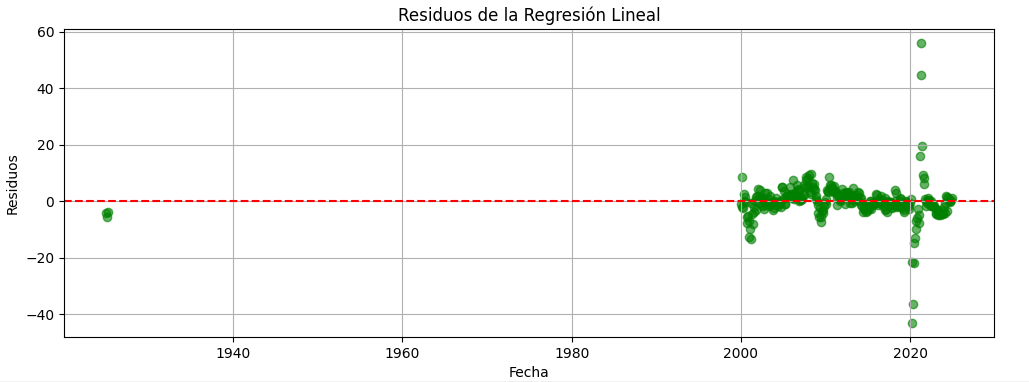
\includegraphics[width=0.5\textwidth]{3grafico.png} % Reemplaza con tu gráfico
        \caption{Distribución de residuos.}
    \end{figure}
\end{frame}

% --- Conclusiones ---
\section{Conclusiones}
\begin{frame}{Conclusiones}
    \begin{itemize}
        \item La regresión lineal muestra una tendencia leve decreciente ($\beta_1 = -0.0474$), pero con bajo poder explicativo ($R^2 = 0.0062$).
        \item Optuna sugiere que un modelo polinomial (grado 5) reduce el MSE en un 6.12\%.
        \item Recomendación:
        \begin{itemize}
            \item Explorar modelos no lineales (ej: ARIMA, Prophet).
            \item Incorporar variables externas (ej: precios de commodities).
        \end{itemize}
    \end{itemize}
\end{frame}

\begin{frame}
    \centering
    \Large ¡Gracias por su atención!\\
    \vspace{1cm}
\end{frame}

\end{document}